\documentclass[journal]{IEEEtran}
\usepackage{amsmath,amssymb}
\usepackage{graphicx}
\usepackage{booktabs}
\usepackage{multirow}
\usepackage{url}
\usepackage{xcolor}
\newcommand{\TODO}[1]{\textcolor{red}{[TODO: #1]}}
\newcommand{\PMten}{PM$_{10}$}
\newcommand{\PMtwo}{PM$_{2.5}$}
\newcommand{\PMone}{PM$_{1}$}

\begin{document}

\title{EnvFiLM: Environment-Conditioned Calibration of Low-Cost Particulate Matter Sensors}

\author{\TODO{Author names and affiliations}}

\maketitle

\begin{abstract}
Low-cost optical particle sensors need a learned calibration, and recent deep-learning calibrators for this task
use attention over the particle signal alone. We show that the sensor boxes already measure the most useful extra
information, their own humidity and temperature and those of the target instrument, and that it works best when it
changes how the particle signal is read rather than entering as one more input. We propose EnvFiLM, a dilated
convolutional calibrator on the log particle signal whose every layer is scaled and shifted by a bounded encoding of
this on-board state (feature-wise linear modulation). On the SensEURCity benchmark of TESLA (AAAI 2025), with the
authors' own data and protocol, EnvFiLM lowers city-averaged RMSE by 43\% to 52\% relative to the published SCARE
results and is lower than published TESLA in all nine city and size cells. Against the same network given exactly
the same channels, it has a lower error on 65.6\% of 195 held-out units over two training seeds (Wilcoxon $p = 1.6\times10^{-6}$), and
removing the modulation makes it worse on 81\% of units. When the target is the station's reference instrument and
each model is averaged over four training seeds, EnvFiLM is better than the same-input network on 83.7\% of 153
units with a 5.4\% lower median error. EnvFiLM is sensitive to its training seed and does not transfer from spring to
the following winter; we report both limitations with the designs that did not help.
\end{abstract}

\begin{IEEEkeywords}
low-cost sensors, particulate matter, sensor calibration, feature-wise linear modulation, temporal convolutional networks, humidity
\end{IEEEkeywords}

\section{Introduction}

Networks of low-cost air-quality sensors can map pollution at a spatial density that regulatory
monitoring stations cannot reach, but the raw readings of optical particle sensors differ from reference
instruments by tens of percent and depend on humidity, temperature and the particles themselves
\cite{karagulian2019,crilley2018,diantonio2018}. A calibration model maps the low-cost reading to the value a
better instrument would report. Statistical and machine-learning calibrations are well established when a
sensor is co-located with a reference \cite{zimmerman2018,malings2019,barkjohn2021,concas2021}, and recent
work treats calibration of minute-resolved signals as a sequence-modelling problem. TESLA \cite{ahn2025}
introduced a benchmark on the public SensEURCity dataset \cite{vanpoppel2023} and a Transformer with
logarithmically binned attention; SCARE \cite{yun2025} improved on it with a compressed bitwise attention.
Both models read only the particle channel.

This paper makes three observations and builds a model on them. First, each SensEURCity box also measures
its own environmental state, including the internal humidity and temperature of the optical particle
counter that the benchmark uses as its target, and this state explains a large share of the remaining
error. Second, a plain dilated convolutional network on the logarithm of the particle signal is a much
stronger baseline than the attention models that define the state of the art on this benchmark. Third,
and this is the modelling contribution, the environmental state works best when it modulates the
particle pathway at every layer rather than entering as an additional input channel or only at the output.

Our contributions are:
\begin{enumerate}
\item EnvFiLM, a calibrator in which an encoder of the on-board state produces a bounded per-channel scale
and shift for every layer of a dilated convolutional network on the log particle signal
(Section~\ref{sec:method}).
\item A comparison on the TESLA benchmark using the authors' own preprocessed files, with equal-information
baselines (TESLA and a convolutional network given the same channels), a capacity-matched control and an
ablation that switches the modulation off (Section~\ref{sec:results}).
\item A unit-rotation protocol in which every unit is held out once, used as the primary test of the
architecture because the official protocol has a single test unit per city
(Section~\ref{sec:protocol}).
\item A second benchmark on the same units in which the target is the station's reference instrument,
where the architectural advantage is larger, and a statement of the conditions in which EnvFiLM does not
help (Sections~\ref{sec:ref} and \ref{sec:limits}).
\end{enumerate}
All design decisions were taken on training or validation units, and the pass criteria of every
confirmatory test were written down before the test was run.

\section{Related Work}

\textit{Calibration of low-cost particle sensors.} Linear and multivariate regressions with humidity
terms, random forests and neural networks are standard for co-located calibration
\cite{zimmerman2018,malings2019,barkjohn2021,karagulian2019,concas2021}. Physically motivated corrections
model hygroscopic growth of particles at high relative humidity \cite{diantonio2018,crilley2018,petters2007}.
The closest learned approach to ours is the neural correction of Koziel et al. \cite{koziel2025}, in which a
network maps temperature, humidity and the raw reading to a multiplicative and an additive correction of the
output. EnvFiLM differs in where the environment acts: it modulates the internal features of a temporal
network at every layer, and our ablation shows that environmental information delivered only at the output
is clearly worse (Section~\ref{sec:ablation}).

\textit{Fine-grained sequence calibration.} TESLA \cite{ahn2025} and SCARE \cite{yun2025} frame calibration
of one-minute signals as sequence regression over a 360-minute window and design attention mechanisms that
fit microcontrollers; their baselines include linear models, PatchTST \cite{nie2023}, iTransformer
\cite{liu2024} and Mamba. Simple models have repeatedly been found competitive with Transformers on time-series
tasks \cite{zeng2023}. Dilated convolutional networks \cite{oord2016,bai2018} were not among the baselines of
either benchmark paper.

\textit{Conditioning.} Feature-wise linear modulation (FiLM) \cite{perez2018} conditions a network by
predicting a per-channel scale and shift from a side input. We did not find prior use of feature-level
environmental conditioning in low-cost sensor calibration.

\section{Problem and Benchmarks}
\label{sec:problem}

\textit{TESLA benchmark.} SensEURCity \cite{vanpoppel2023} contains one-minute data from 85 AirSensEUR boxes in
Antwerp, Oslo and Zagreb. TESLA \cite{ahn2025} uses each box's first co-location period at a reference station,
takes a Plantower PMS5003 channel as the low-cost input and the box's Alphasense OPC-N3 reading of the same size
fraction (\PMten, \PMtwo{} or \PMone) as the target, and splits by unit: in each city the units are kept in a
fixed order, the last one tests, the second-to-last validates and the rest train. The model sees the previous
360 rows of the input and predicts the target at the last row; the metric is RMSE in \textmu g/m$^3$. We use
the authors' preprocessed files (row counts identical to their Table A1) and their unit lists. Rows were dropped by
the authors wherever a value or a quality flag was missing, so consecutive rows are not always consecutive minutes;
windows are taken over rows, as in the original code. Table~\ref{tab:data} summarises the benchmark.

\begin{table}[t]
\centering
\caption{The TESLA benchmark as used here (authors' preprocessed files). Units are split in the authors' order: all
but the last two train, the second-to-last validates, the last tests.}
\label{tab:data}
\begin{tabular}{lrrl}
\toprule
City & Units & Rows (minutes) & First co-location period \\
\midrule
Antwerp & 30 & 3,113,955 & 2020-04-03 to 2020-06-15 \\
Oslo & 21 & 810,314 & 2020-09-17 to 2020-10-14 \\
Zagreb & 14 & 939,838 & 2020-05-22 to 2020-07-08 \\
\bottomrule
\end{tabular}
\end{table}

\textit{On-board state.} Each box also records ambient relative humidity and temperature (SHT31) and the OPC-N3
reports its own internal humidity and temperature. We attach these four channels to the authors' rows by
timestamp. They are measured inside the box at deployment, so using them requires no extra instrument.

\textit{True-reference benchmark.} To test whether the conclusions depend on calibrating against a second
low-cost sensor, we build a variant on the same units and periods in which the target is the station's
reference instrument (FIDAS in Antwerp, the station reference in Oslo); because not all references are
minute-resolved, all signals are averaged to 10 minutes and the window is 36 steps (the same six hours).
Zagreb is excluded because its reference is not sub-hourly. The unit lists and splits are those of the TESLA
benchmark.

\section{EnvFiLM}
\label{sec:method}

\textit{Motivation.} Humidity and temperature do not add a fixed amount to an optical particle reading. Water uptake
changes particle size and refractive index, so its effect on a light-scattering sensor scales with the particle signal
and depends on the size distribution \cite{diantonio2018,crilley2018,petters2007}; the two sensors of a SensEURCity box
also sit in the same housing and share its temperature. A model that simply receives humidity as one more input must
learn such multiplicative interactions from data. Feature-wise linear modulation \cite{perez2018} builds them in: the
side input sets a gain and an offset for every feature channel, so the environment can change how strongly each learned
temporal pattern of the particle signal contributes to the output.

Fig.~\ref{fig:arch} shows the model. The particle window $x_{t-N+1},\dots,x_t$ is transformed to
$\ell = \log(1 + x)$, because concentrations are heavy-tailed and optical sensor responses are closer to
multiplicative than additive. Seven convolution layers with kernel size 3, 32 channels and dilations
$1, 2, \dots, 64$ cover the window. The on-board state window $e \in \mathbb{R}^{N\times 4}$ is standardised
with training statistics and clipped to $\pm3$ standard deviations. A summary vector $z$ concatenates, for each
channel, the last value, the window mean, the change over the last hour, and the window minimum and maximum. An
environment encoder (two-layer MLP with 64 hidden units) maps $z$ to a scale $\gamma_k$ and shift $\beta_k$ for
every channel of every layer $k$:
\begin{equation}
h_k = \mathrm{GELU}\big( (1 + \tfrac12\tanh \gamma_k) \odot \mathrm{Conv}_k(h_{k-1}) + \tfrac12 \tanh \beta_k \big).
\end{equation}
The encoder's last layer is initialised at zero, so training starts from an unconditioned network. The bound
keeps every scale in $[0.5, 1.5]$; Section~\ref{sec:limits} shows why it is necessary. The head is an MLP on
the last and mean states of the final layer, the last value of $\ell$, and $z$. EnvFiLM has 54,785 parameters;
Table~\ref{tab:hyper} lists the configuration. The output is in the scale of the target (divided by 300, as in the
original code) and the loss is the mean squared error.

\begin{table}[t]
\centering
\caption{EnvFiLM configuration (identical on both benchmarks; not tuned on test units).}
\label{tab:hyper}
\begin{tabular}{ll}
\toprule
Component & Setting \\
\midrule
Input transform & $\log(1 + x)$, $x$ in \textmu g/m$^3$ \\
Convolutions & 7 layers, kernel 3, 32 channels, dilations $2^0..2^6$, GELU \\
State channels & ambient RH and $T$, OPC-N3 internal RH and $T$ \\
State summary $z$ & last, mean, change over last 60 steps, min, max \\
State clipping & $\pm3$ training standard deviations \\
Environment encoder & MLP $20 \to 64 \to 2\cdot 32\cdot 7$, last layer zero-initialised \\
Modulation & scale $1+\frac12\tanh\gamma$, shift $\frac12\tanh\beta$ \\
Head & MLP on [last state, mean state, last $\ell$, $z$], 64 hidden units \\
Training & Adam, lr $10^{-3}$, batch 512, 10 epochs, best validation epoch \\
\bottomrule
\end{tabular}
\end{table}

\begin{figure*}[t]
\centering
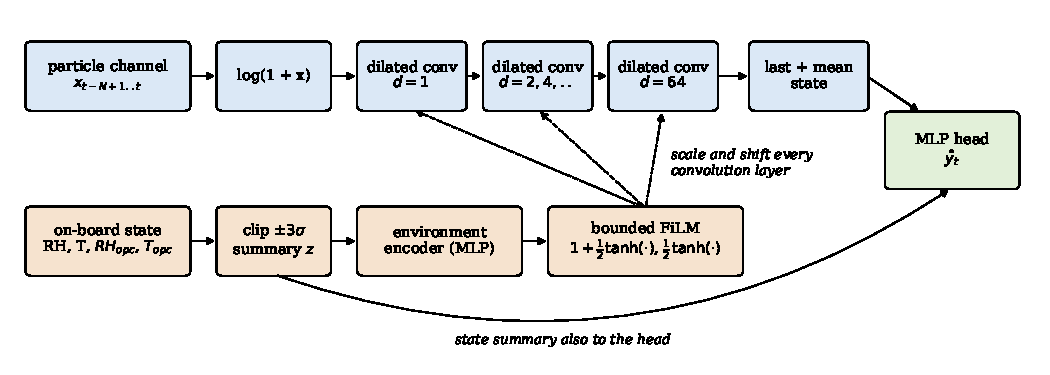
\includegraphics[width=0.85\textwidth]{fig_arch.pdf}
\caption{EnvFiLM. A dilated convolutional network reads the log particle signal; an encoder of the on-board state
(ambient and target-instrument humidity and temperature) produces a bounded scale and shift for every convolution
layer, and its summary also reaches the output head.}
\label{fig:arch}
\end{figure*}

\section{Experimental Protocol}
\label{sec:protocol}

\textit{Baselines.} All models are trained with the same recipe (Adam, learning rate $10^{-3}$, batch 512, 10
epochs, mean squared error, best epoch on the validation unit):
\begin{itemize}
\item TESLA, our PyTorch re-implementation of the official code, and published TESLA and SCARE numbers;
\item TESLA + env.: TESLA with the four state channels concatenated to the particle value before its token
embedding (equal information);
\item LogTCN: the EnvFiLM convolution stack and head without any environmental input;
\item TCN + env.: LogTCN with the four state channels as additional input channels at every time step (equal
information, early fusion);
\item TCN + env., size-matched: the same with 50 channels (52,949 parameters, matched to EnvFiLM);
\item EnvFiLM, modulation off: EnvFiLM with the FiLM path removed, so the state summary reaches only the head.
\end{itemize}
Our TESLA re-implementation reproduces the published numbers closely on the authors' data (for example \PMten{}
14.09 versus 14.58 in Antwerp and 13.53 versus 13.87 in Zagreb).

\textit{Official split.} Three seeds per model and cell; we report the mean.

\textit{Unit rotation.} The official protocol tests one unit per city, and we measured run-to-run differences
of the order of 7\% on a single unit with an identical seed (GPU non-determinism), comparable to the effects of
interest. We therefore also hold out every unit once: per city and size fraction the unit list is cut into
five folds; a fold's units test, two other units validate, the rest train (every fourth window, for all models
alike). The comparison with the same-input TCN uses per-unit RMSE averaged over two training seeds on the TESLA benchmark and four on the true-reference benchmark; the comparison with the modulation switched off uses one seed. This gives 195 unit cases on the TESLA benchmark and 153 on the true-reference benchmark. We
report the share of units on which EnvFiLM has the lower RMSE, the median ratio of per-unit RMSEs, a sign test
and a Wilcoxon signed-rank test on log ratios.

\textit{Development and pre-registration.} Model components were chosen on a development protocol that uses
only the official training units (four folds of held-out training units). Before each confirmatory run we wrote
down its pass criteria; the main criterion for the architecture was the rotation test (better on at least 55\%
of units with a pooled median ratio below one). An earlier criterion defined on the official split alone, set for the
unbounded variant of Section~\ref{sec:limits}, was narrowly missed; together with the single-unit noise described
above, this is why the rotation is our primary test.

\section{Results}
\label{sec:results}

\subsection{TESLA benchmark}

Table~\ref{tab:main} gives the official-split results. EnvFiLM is lower than published TESLA in all nine cells
(mean ratio 0.54) and lower than our TESLA re-implementation in all nine. Averaged over cities, its RMSE is
8.04 (\PMten), 2.71 (\PMtwo) and 1.36 (\PMone), against 14.03, 5.67 and 2.51 reported for SCARE and 14.75, 6.16
and 3.18 for TESLA. Against the equal-information baselines, EnvFiLM is lower in 6 of 9 cells than the TCN with
the same channels (mean ratio 0.95), in 7 of 9 than its size-matched version (0.97) and in 7 of 9 than TESLA with
the same channels (0.79).

\begin{table*}[t]
\centering
\caption{RMSE (\textmu g/m$^3$) on the TESLA benchmark (authors' data, official split, mean of three seeds;
published TESLA from \cite{ahn2025}, one value per cell). Columns 2 to 4 receive the same four on-board state
channels as EnvFiLM. Best per row in bold.}
\label{tab:main}
\begin{tabular}{llrrrrrrr}
\toprule
PM & City & \rotatebox{90}{EnvFiLM (ours)} & \rotatebox{90}{TCN + env. channels} & \rotatebox{90}{TCN + env., size-matched} & \rotatebox{90}{TESLA + env. channels} & \rotatebox{90}{LogTCN (particles only)} & \rotatebox{90}{TESLA (our re-impl.)} & \rotatebox{90}{TESLA (published)} \\
\midrule
PM$_{10}$ & Antwerp & \textbf{6.43} & 6.67 & 6.77 & 9.53 & 10.53 & 14.09 & 14.58 \\
PM$_{10}$ & Oslo & \textbf{8.16} & 8.74 & 8.95 & 10.46 & 11.30 & 14.46 & 15.79 \\
PM$_{10}$ & Zagreb & \textbf{9.52} & 10.29 & 9.62 & 11.54 & 10.29 & 13.53 & 13.87 \\
PM$_{2.5}$ & Antwerp & \textbf{2.31} & 2.86 & 2.62 & 5.80 & 6.25 & 7.09 & 7.54 \\
PM$_{2.5}$ & Oslo & \textbf{3.10} & 3.45 & 3.37 & 3.88 & 3.99 & 6.79 & 7.90 \\
PM$_{2.5}$ & Zagreb & 2.72 & 2.60 & 2.84 & \textbf{2.53} & 2.57 & 2.99 & 3.03 \\
PM$_{1}$ & Antwerp & 1.68 & 1.60 & \textbf{1.38} & 2.60 & 2.90 & 4.71 & 4.78 \\
PM$_{1}$ & Oslo & \textbf{1.32} & 1.73 & 1.48 & 2.09 & 1.88 & 3.14 & 3.63 \\
PM$_{1}$ & Zagreb & 1.07 & 0.95 & 1.02 & \textbf{0.84} & 0.97 & 1.35 & 1.14 \\
\bottomrule
\end{tabular}

\end{table*}

Part of the gain over the published models comes from the information in the on-board channels: LogTCN, which
does not use them, already improves on published TESLA in all nine cells, and adding the channels as inputs
helps further. On the development protocol, ambient humidity alone lowered the per-unit RMSE of LogTCN on 79.7\%
of 118 held-out training units (median ratio 0.91), and the four channels improved on humidity alone on 79.0\%
of 62 (median 0.93). The oracle analysis of Section~\ref{sec:limits} explains why: the ratio between the two
sensors moves from day to day with an interquartile range of 45\% of its median, and the daily ratio correlates
with humidity and with the concentration level.

\subsection{Is it the architecture or the information?}
\label{sec:ablation}

The official split cannot separate effects of a few percent. The unit rotation can
(Fig.~\ref{fig:rot}). Over 195 held-out units, EnvFiLM is better than the TCN with the same four channels on
65.6\% of units when each unit's RMSE is averaged over two training seeds (bootstrap 95\% interval over units 59.0\% to
72.3\%), with a median per-unit ratio of 0.974 (interval 0.960 to 0.984; sign test $p = 1.5\times10^{-5}$; Wilcoxon
$p = 1.6\times10^{-6}$), and its mean RMSE is lower in six of the nine city and size groups (Table~\ref{tab:groups}).
Each seed on its own also favours EnvFiLM: 62.6\% of units with median ratio 0.967 for the first and 59.0\% with 0.984
for the second. In the three Zagreb groups the median unit favours EnvFiLM but a few units with large errors raise its
mean. Against the same model with the modulation
switched off, EnvFiLM is better on 81.0\% of units (interval 75.4\% to 86.2\%; median ratio 0.912, interval 0.890 to
0.928; Wilcoxon $p = 6.7\times10^{-17}$): the environment is far more useful when it changes the particle pathway than
when it reaches only the output head. The comparison with the TCN given the same channels is closer, because that
model also lets the environment interact with the particle signal from the first layer on; EnvFiLM's advantage is that
the interaction is multiplicative and conditioned on a summary of the whole window rather than learned implicitly from
concatenated channels.

\begin{table*}[t]
\centering
\caption{Unit rotation by group: number of held-out units on which EnvFiLM has the lower RMSE, and the median ratio of
per-unit RMSEs (EnvFiLM / comparison; below one favours EnvFiLM). TESLA benchmark: against the TCN with channels, per-unit RMSE averaged over two seeds; against the modulation switched off, one seed; true reference: per-unit
RMSE averaged over four seeds. Zagreb has no sub-hourly reference instrument.}
\label{tab:groups}
\begin{tabular}{llrrrrrr}
\toprule
 & & \multicolumn{2}{c}{TESLA bench., vs TCN+env.} & \multicolumn{2}{c}{TESLA bench., vs mod. off} & \multicolumn{2}{c}{True ref., vs TCN+env.} \\
PM & City & better & median & better & median & better & median \\
\midrule
PM$_{10}$ & Antwerp & 16/30 & 0.990 & 28/30 & 0.897 & 30/30 & 0.915 \\
PM$_{10}$ & Oslo & 9/21 & 1.020 & 15/21 & 0.929 & 16/21 & 0.974 \\
PM$_{10}$ & Zagreb & 11/14 & 0.956 & 12/14 & 0.960 & n/a & n/a \\
PM$_{2.5}$ & Antwerp & 18/30 & 0.970 & 26/30 & 0.877 & 26/30 & 0.946 \\
PM$_{2.5}$ & Oslo & 14/21 & 0.942 & 10/21 & 1.033 & 18/21 & 0.939 \\
PM$_{2.5}$ & Zagreb & 12/14 & 0.962 & 12/14 & 0.962 & n/a & n/a \\
PM$_{1}$ & Antwerp & 20/30 & 0.957 & 25/30 & 0.865 & 24/30 & 0.940 \\
PM$_{1}$ & Oslo & 13/21 & 0.869 & 18/21 & 0.820 & 14/21 & 0.975 \\
PM$_{1}$ & Zagreb & 9/14 & 0.942 & 12/14 & 0.873 & n/a & n/a \\
\midrule
All & & 122/195 & 0.967 & 158/195 & 0.912 & 128/153 & 0.946 \\
\bottomrule
\end{tabular}

\end{table*} Size does not explain the gain: on the development protocol EnvFiLM was better than
the size-matched TCN on 68.8\% of 93 units (median 0.951).

\begin{figure}[t]
\centering
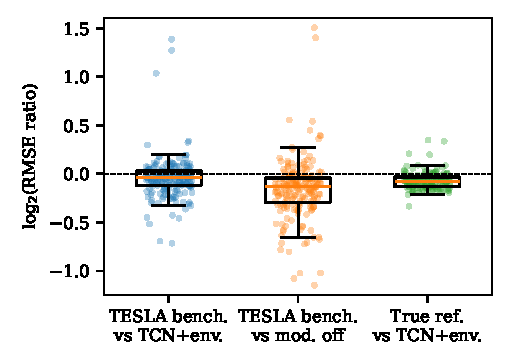
\includegraphics[width=\columnwidth]{fig_rotation.pdf}
\caption{Per-unit log$_2$ RMSE ratios of EnvFiLM against the TCN with the same channels and against EnvFiLM with
the modulation switched off (TESLA benchmark, 195 units; two seeds against the TCN, one against the modulation switched off), and against the TCN with the same channels on the
true-reference benchmark (153 units, per-unit RMSE averaged over four seeds). Values below zero favour EnvFiLM; every
unit is shown.}
\label{fig:rot}
\end{figure}

\subsection{True-reference benchmark}
\label{sec:ref}

Table~\ref{tab:ref} reports the official split of the true-reference benchmark with unchanged models and
hyperparameters (at 10-minute resolution the ``last hour'' change in $z$ spans the whole window; we left the
feature unchanged). EnvFiLM has the lowest error in five of six cells and is tied in the sixth (\PMtwo{} Oslo, 1.40
versus 1.39). It is lower than TESLA and than TESLA with the same channels in all six cells (mean ratios 0.45 and
0.48). Because this rotation is fast, we repeated it with four training seeds. Averaging each unit's RMSE over the
four seeds for each model, EnvFiLM is better than the TCN with the same channels on 83.7\% of 153 units (bootstrap
95\% interval 77.8\% to 89.5\%), with a median ratio of 0.946 (interval 0.939 to 0.957; Wilcoxon
$p = 1.8\times10^{-17}$) and a lower mean in five of six groups. The individual seeds are bimodal: two give a clear
advantage (better on 88.9\% and 88.2\% of units, median ratios 0.893 and 0.896) and two are tied with the TCN (51.6\%
and 49.0\%, median ratios 0.997 and 1.002); none is worse. We discuss this training sensitivity in
Section~\ref{sec:limits}. A plausible reason why the advantage is larger and more uniform here than on the TESLA
benchmark is that the reference instrument is shared by all units, so the unit-specific gain of the low-cost target
sensor, which no input can reveal (Section~\ref{sec:limits}), no longer dominates the error, and the multiplicative
humidity effect on optical sensors is what the modulation can represent.

\begin{table}[t]
\centering
\caption{RMSE (\textmu g/m$^3$) on the true-reference benchmark (10-minute data, official split, mean of three
seeds). Best per row in bold.}
\label{tab:ref}
\resizebox{\columnwidth}{!}{\begin{tabular}{llrrrrr}
\toprule
PM & City & EnvFiLM (ours) & TCN + env. channels & TESLA + env. channels & LogTCN (particles only) & TESLA (particles only) \\
\midrule
PM$_{10}$ & Antwerp & \textbf{4.96} & 5.18 & 8.59 & 8.10 & 9.11 \\
PM$_{10}$ & Oslo & \textbf{3.10} & 3.58 & 6.11 & 5.85 & 7.29 \\
PM$_{2.5}$ & Antwerp & \textbf{2.17} & 2.87 & 6.15 & 3.58 & 5.35 \\
PM$_{2.5}$ & Oslo & 1.40 & \textbf{1.39} & 2.44 & 2.10 & 2.75 \\
PM$_{1}$ & Antwerp & \textbf{2.05} & 2.48 & 6.02 & 3.56 & 5.80 \\
PM$_{1}$ & Oslo & \textbf{1.27} & 1.31 & 2.49 & 1.88 & 2.84 \\
\bottomrule
\end{tabular}
}
\end{table}

\subsection{Cost}

EnvFiLM has 54,785 parameters, against 23,681 for the TCN with channels and 4,531 for TESLA with channels. A
single 360-minute window takes 2.9 ms on one CPU core in PyTorch, against 1.9 ms and 1.0 ms. EnvFiLM is therefore
larger than the microcontroller-oriented TESLA and SCARE designs; we have not optimised it for embedded deployment.

\section{Discussion}
\label{sec:discussion}

\textit{Why a convolutional network beats the attention models here.} Our re-implementation of TESLA, trained with the
same recipe as every other model, reproduces the published numbers, so the gap between TESLA and LogTCN is not a matter of
training. Two properties of the benchmark favour the convolutional design. The useful information is local and recent
(the target is the reading at the last minute of the window), which dilated convolutions capture directly and
logarithmic binning of older tokens partly discards; and the input is heavy-tailed, which the log transform handles and
the raw-scale input of TESLA does not. In early exploratory runs on our own reconstruction of the benchmark from the raw archive (before the
authors' files were used), giving TESLA a log-scaled input did not improve it (7.55 versus 7.04 on Oslo \PMtwo), whereas
the same change mattered for the convolutional network (from 5.12 to 4.47), which suggests that the difference lies in the
architecture rather than the scaling alone. This mirrors the broader observation that simpler models
are often competitive with Transformers on time-series tasks \cite{zeng2023}.

\textit{Why modulation helps more against a true reference.} On the TESLA benchmark each unit is compared with its own
OPC-N3, whose unit-specific gain adds an error that no input can explain (Section~\ref{sec:limits}). Against a shared
reference instrument that error disappears, and what remains is closer to the physical problem that motivated the design:
the effect of humidity on the optical response. The larger and more uniform advantage on the true-reference benchmark
(Table~\ref{tab:groups}) is consistent with this reading.

\textit{Practical use.} The four state channels are measured inside every AirSensEUR box, so EnvFiLM needs no additional
hardware. It does need the internal humidity and temperature of the target instrument when it is trained, which is
available in co-location campaigns such as SensEURCity. Its cost per window (2.9 ms on one CPU core) is small for
server-side calibration; it is larger than the microcontroller-oriented designs of TESLA and SCARE.

\section{Limitations and What Did Not Help}
\label{sec:limits}

\textit{Ceiling of the TESLA benchmark.} Fitting, with test labels and only for diagnosis, the best scalar gain per
held-out training unit removes a median of 19\% of the error variance, and the remaining error is still 4.9 times
the minute-to-minute noise of the target. Across co-located units the gains of the input sensors relative to the fleet have an interquartile range of about
$\pm3\%$, those of the OPC-N3 targets about $\pm10$ to 15\%, so a part of the error on this benchmark belongs to the target
instrument and cannot be predicted from any input.

\textit{Seasons.} We trained on the first co-location (spring 2020) and tested on each unit's second co-location
eight to ten months later. All models' errors grow, by factors between 1.2 and 5.4 for the TCN with channels (for
example \PMten{} in Antwerp from 6.7 to 26.2), and the sensor-to-sensor ratio itself shifts by up to $\pm50\%$ between the
two periods. EnvFiLM does not help there: it is better than the TCN with the same channels on 35.9\% of 128 units
(median ratio 1.034).

\textit{Sensitivity to the training seed.} On the true-reference benchmark, two of four training seeds gave EnvFiLM a
clear advantage and two left it tied with the TCN that receives the same channels, while the TCN itself varied little
between seeds (median seed-to-seed ratio 0.98 against 1.09 for EnvFiLM between the first two seeds). The modulation path
starts at zero and appears not to engage in every run within the ten-epoch budget. We therefore recommend averaging
several trainings; selecting, per fold, the seed with the lowest validation error recovered less of the advantage
(73.2\% of units, median ratio 0.951) than averaging (83.7\%, 0.946). On the TESLA benchmark the seed effect was
smaller: both seeds favoured EnvFiLM (62.6\% and 59.0\% of units), and averaging the two gave 65.6\%.

\textit{Bounded modulation is necessary.} An unbounded version of EnvFiLM (scale $1 + \gamma$, no input clipping)
performed similarly in season (better than the TCN with channels on 67.7\% of 195 units) but failed badly out of
season, where conditions leave the training range: its median per-unit ratio to the TCN with channels was 11.4 and
the worst unit 111. With the bound the worst unit was 1.26.

\textit{Designs that did not help.} On the development protocol we also tested a physically shaped humidity gate
following the $\kappa$-K\"ohler growth law \cite{petters2007} (better than the TCN with humidity on 40\% of units,
median ratio 1.05), a latent gain per training unit's target sensor (44\%, 1.01), residual blocks with dropout,
multi-scale input and a log-normal output head (residual blocks better on 3\% of units, median 1.11), a
multiplicative gain head with a label-free context of the unit's own recent readings and gain augmentation, and
self-supervised joint-embedding pretraining of the convolution trunk on 32 million unlabelled minutes from the
whole fleet \cite{assran2023,bardes2022}, as initialisation, as a joint objective, as frozen features and with a
reduced learning rate. None improved on the plain network on validation units, and the pretrained variants were
worse in every cell tested.

\textit{Threats to validity.} The official split has one test unit per city, and identical seeds can differ by about 7\%
on a single unit because GPU training is not bit-reproducible; we therefore rest the architectural claim on the unit
rotation. The rotation uses two to four training seeds for the main comparison, one for the ablation, and every fourth training window for all models alike. The on-board channels
are attached to the authors' rows by timestamp from the SensEURCity archive; rows without them were interpolated within each
unit. Our TESLA re-implementation follows the official TensorFlow code in PyTorch with identical sizes; SCARE is cited from
its paper only.

\textit{Scope.} All results are on SensEURCity. We make no claim about other sensor platforms or networks.

\section{Conclusion}

On the TESLA benchmark, the most useful information for calibrating a low-cost particle sensor is already inside the
sensor box, and the most useful way to use it is to let it modulate how the particle signal is read. EnvFiLM, a
dilated convolutional calibrator with bounded feature-wise environmental modulation, lowers the error of the published
attention-based models by about half and beats an equal-information convolutional network on most held-out units, by
a larger margin when the target is a true reference instrument. The remaining problem is change between seasons,
which neither EnvFiLM nor the baselines solve.

\section*{Data and Code Availability}
SensEURCity is available from Zenodo \cite{vanpoppel2023}; the TESLA preprocessed files from the authors' repository
\cite{ahn2025}. Code, result files and the pre-registration notes are available from the authors on request
\TODO{repository link when made public}.

\begin{thebibliography}{99}

\bibitem{karagulian2019} F.~Karagulian \emph{et al.}, ``Review of the performance of low-cost sensors for air quality
monitoring,'' \emph{Atmosphere}, vol.~10, no.~9, p.~506, 2019.

\bibitem{crilley2018} L.~R.~Crilley \emph{et al.}, ``Evaluation of a low-cost optical particle counter (Alphasense
OPC-N2) for ambient air monitoring,'' \emph{Atmos. Meas. Tech.}, vol.~11, pp.~709--720, 2018.

\bibitem{diantonio2018} A.~Di~Antonio, O.~A.~M.~Popoola, B.~Ouyang, J.~Saffell, and R.~L.~Jones, ``Developing a
relative humidity correction for low-cost sensors measuring ambient particulate matter,'' \emph{Sensors}, vol.~18,
no.~9, p.~2790, 2018.

\bibitem{zimmerman2018} N.~Zimmerman \emph{et al.}, ``A machine learning calibration model using random forests to
improve sensor performance for lower-cost air quality monitoring,'' \emph{Atmos. Meas. Tech.}, vol.~11, pp.~291--313,
2018.

\bibitem{malings2019} C.~Malings \emph{et al.}, ``Development of a general calibration model and long-term performance
evaluation of low-cost sensors for air pollutant gas monitoring,'' \emph{Atmos. Meas. Tech.}, vol.~12, pp.~903--920,
2019.

\bibitem{barkjohn2021} K.~K.~Barkjohn, B.~Gantt, and A.~L.~Clements, ``Development and application of a United
States-wide correction for PM$_{2.5}$ data collected with the PurpleAir sensor,'' \emph{Atmos. Meas. Tech.}, vol.~14,
pp.~4617--4637, 2021.

\bibitem{concas2021} F.~Concas \emph{et al.}, ``Low-cost outdoor air quality monitoring and sensor calibration: A
survey and critical analysis,'' \emph{ACM Trans. Sensor Netw.}, vol.~17, no.~2, 2021.

\bibitem{ahn2025} S.~Ahn, H.~Kim, S.~Shin, and Y.-D.~Seo, ``Real-time calibration model for low-cost sensor in
fine-grained time series,'' in \emph{Proc. AAAI Conf. Artif. Intell.}, vol.~39, 2025, pp.~3--11.

\bibitem{yun2025} J.~Yun, H.~Kim, S.~Ahn, E.~Lee, and Y.-D.~Seo, ``Sensor calibration model balancing accuracy,
real-time, and efficiency,'' arXiv:2511.06715, 2025.

\bibitem{vanpoppel2023} M.~Van~Poppel \emph{et al.}, ``SensEURCity: A multi-city air quality dataset collected for
2020/2021 using open low-cost sensor systems,'' \emph{Sci. Data}, vol.~10, p.~322, 2023.

\bibitem{koziel2025} S.~Koziel, A.~Pietrenko-Dabrowska, M.~Wojcikowski, and B.~Pankiewicz, ``Efficient field
correction of low-cost particulate matter sensors using machine learning, mixed multiplicative/additive scaling and
extended calibration inputs,'' \emph{Sci. Rep.}, vol.~15, p.~18573, 2025.

\bibitem{petters2007} M.~D.~Petters and S.~M.~Kreidenweis, ``A single parameter representation of hygroscopic growth
and cloud condensation nucleus activity,'' \emph{Atmos. Chem. Phys.}, vol.~7, pp.~1961--1971, 2007.

\bibitem{nie2023} Y.~Nie, N.~H.~Nguyen, P.~Sinthong, and J.~Kalagnanam, ``A time series is worth 64 words: Long-term
forecasting with Transformers,'' in \emph{Proc. ICLR}, 2023.

\bibitem{liu2024} Y.~Liu \emph{et al.}, ``iTransformer: Inverted Transformers are effective for time series
forecasting,'' in \emph{Proc. ICLR}, 2024.

\bibitem{zeng2023} A.~Zeng, M.~Chen, L.~Zhang, and Q.~Xu, ``Are Transformers effective for time series forecasting?''
in \emph{Proc. AAAI Conf. Artif. Intell.}, vol.~37, 2023, pp.~11121--11128.

\bibitem{oord2016} A.~van~den~Oord \emph{et al.}, ``WaveNet: A generative model for raw audio,'' arXiv:1609.03499,
2016.

\bibitem{bai2018} S.~Bai, J.~Z.~Kolter, and V.~Koltun, ``An empirical evaluation of generic convolutional and
recurrent networks for sequence modeling,'' arXiv:1803.01271, 2018.

\bibitem{perez2018} E.~Perez, F.~Strub, H.~de~Vries, V.~Dumoulin, and A.~Courville, ``FiLM: Visual reasoning with a
general conditioning layer,'' in \emph{Proc. AAAI Conf. Artif. Intell.}, vol.~32, 2018.

\bibitem{assran2023} M.~Assran \emph{et al.}, ``Self-supervised learning from images with a joint-embedding predictive
architecture,'' in \emph{Proc. IEEE/CVF CVPR}, 2023.

\bibitem{bardes2022} A.~Bardes, J.~Ponce, and Y.~LeCun, ``VICReg: Variance-invariance-covariance regularization for
self-supervised learning,'' in \emph{Proc. ICLR}, 2022.

\end{thebibliography}

\end{document}
